\section{3 Dimensional Analysis}
\noindent This section is an extended analysis of the 2-dimensional analyses intended to explore and analyse the 3-dimensional flow feature. It was surmised that the 3-dimensional flow offers a complex flow behaviour that may significantly affect an undertray's overall performance. This part of the paper will be divided into 3D open-flow and undertray prototype with bluff body analyses.


\subsection{3D Open-Flow}
This analysis is an extension of the 3-dimensional analysis of 2D open-flow. The purpose of this analysis to investigate further the flow features of an undertray in a 3-dimensional manner, which plausibly affect its performance based on a similar variable as previous analyses.

\subsubsection{Geometry and Mesh generation}
An identical 2D sketch from geometry 3 - 2D open flow was used, which then extruded to 1 meter of thickness with a skirt on both side of the rear diffuser. The skirts were used to improve flow isolation and generate corner vortices which help to improve flow attachment at the diffuser region. Fences were also added to the next analyses to investigate the effect of vortex generator respective to the downforce generation. Geometry sketch can be seen in figure \ref{fig:3D_OF_GEOM} below. 

\begin{figure}[!h]
    \centering
    \noindent\makebox[\textwidth]{
    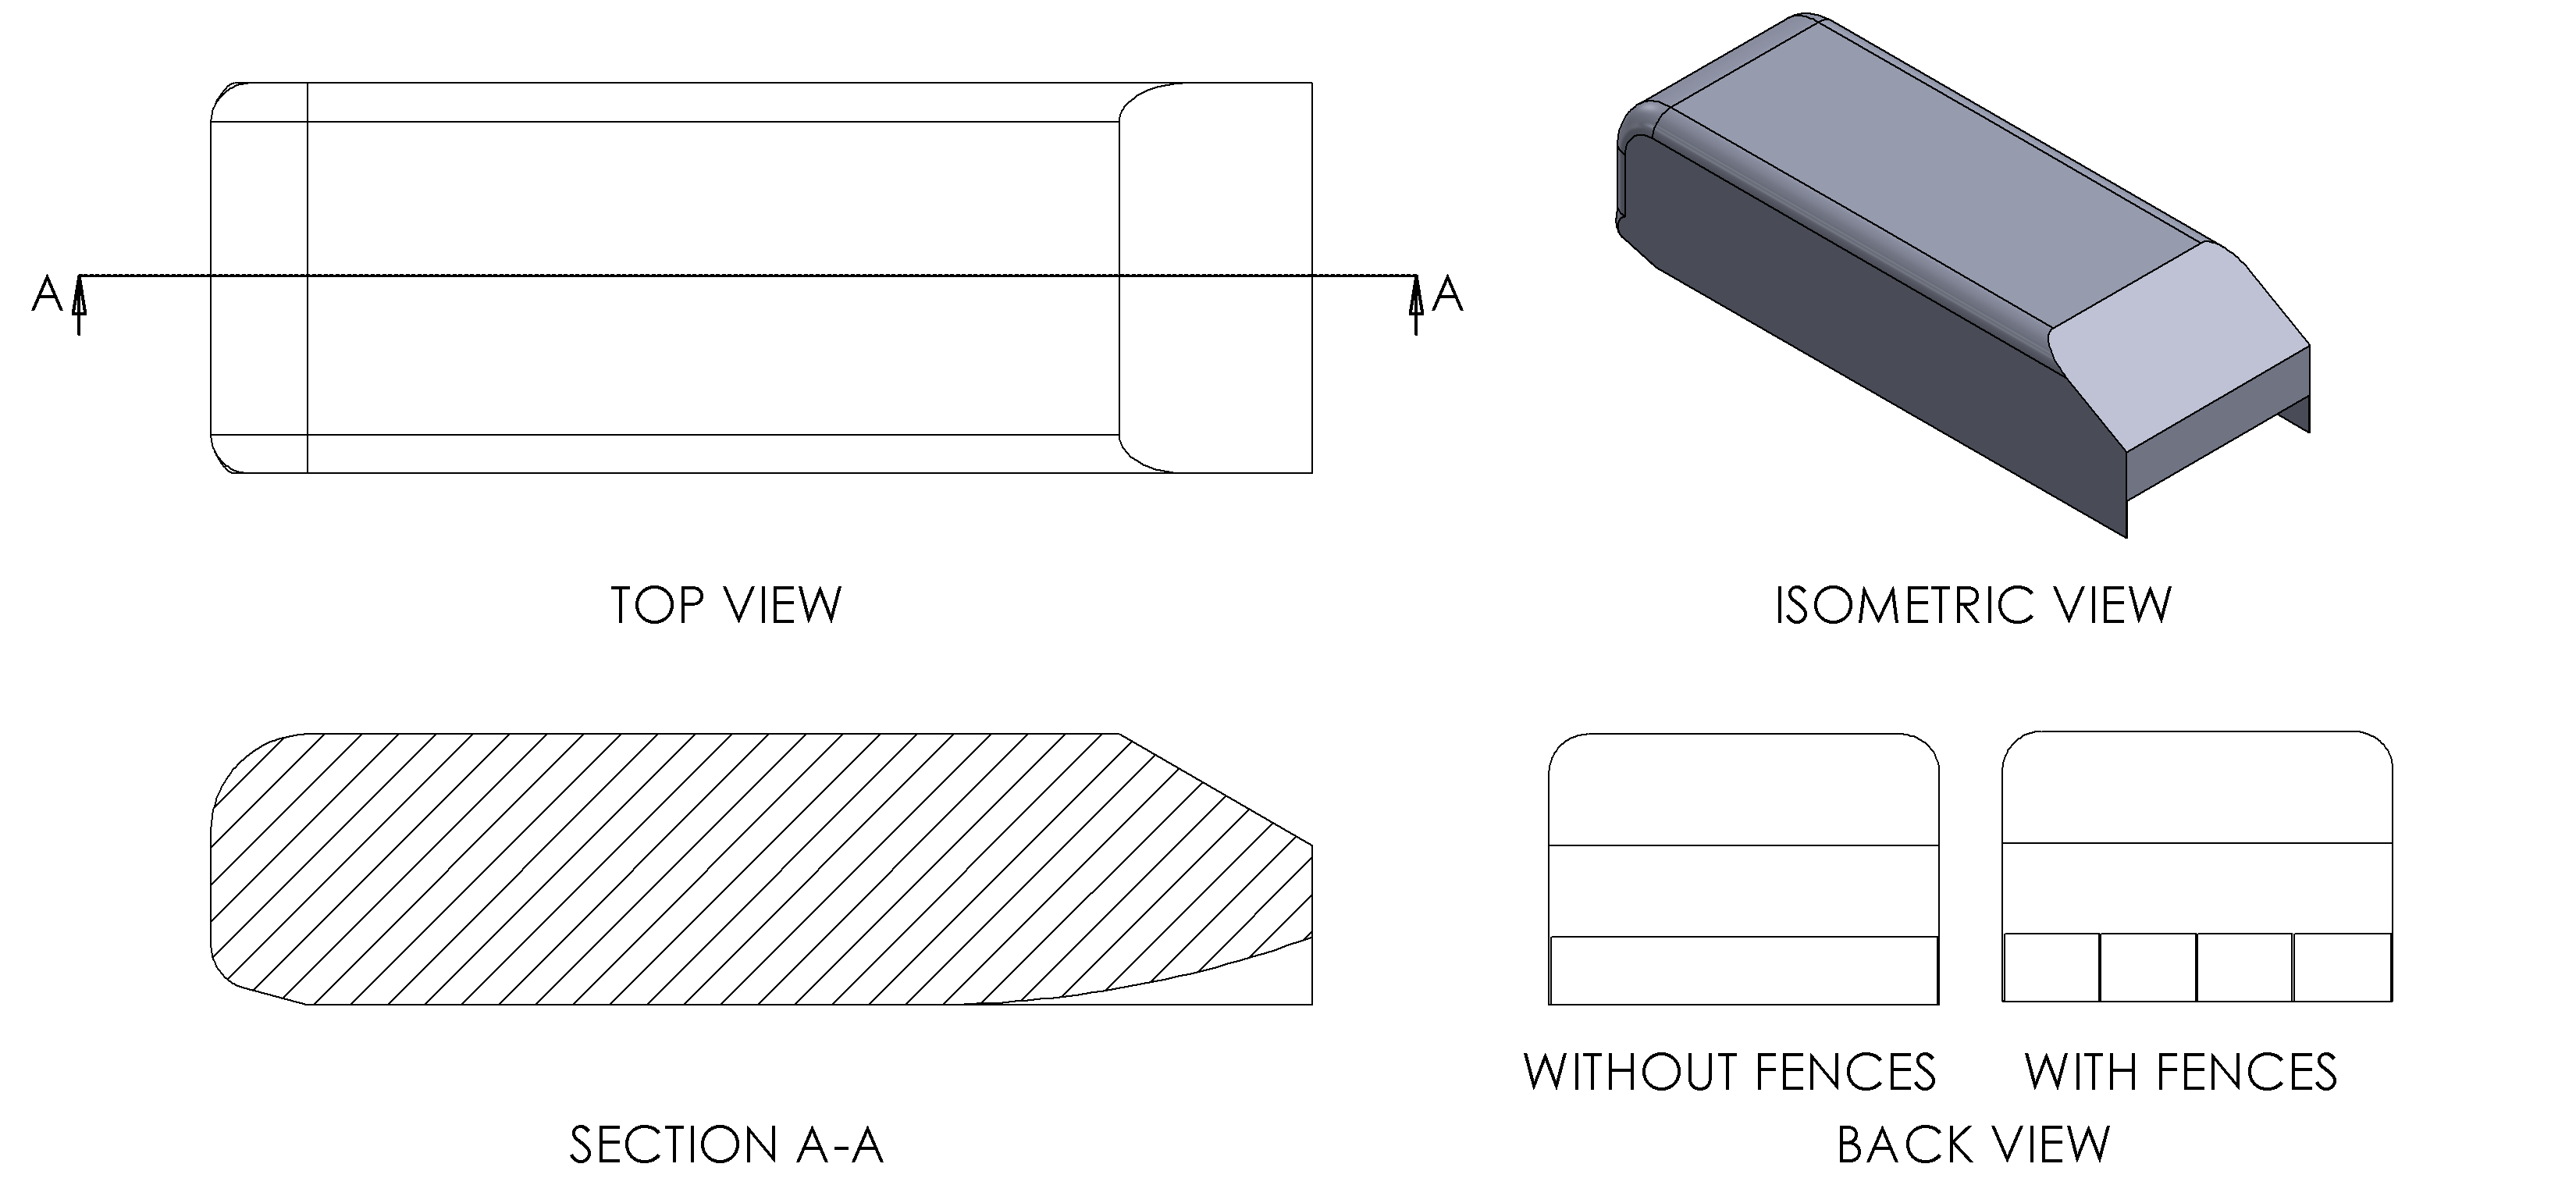
\includegraphics[width=0.8\textwidth]{Figures/3D_OF/3D_OF_D.PNG}}
    \caption{Geometry generated for 3D open-flow analysis.}
    \label{fig:3D_OF_GEOM}
\end{figure}

\noindent The geometry then was imported to the design modeller where fluid domain and body of influence were made. The fluid flow was made 12 meters behind, 5 meters forward, 2 meters top, 0.03 meters bottom, and 1.5 meters wide. Due to the body's symmetry, a partial model was used to create a fluid domain to compress the mesh number. Body of influence (BOI) with a dimension of  6 $\times$1 $\times$ 7 meters were created using box feature around the body to improve the mesh quality and capture the surrounding flow features.  

\noindent A hybrid mesh was used, which comprises a tetrahedron and triangular prisms; therefore, construct 20 inflation layer of triangular prism near the wall with y$^+$=1.  Mesh element size of 0.8 meters and 0.02 meters of BOI generated 1.3 to 1.5 million mesh elements for this analysis. This section's mesh quality is considerably acceptable with average skewness of 1.9 and an aspect ratio of 80-90; however, an extreme jump size in the cell between the inflation layer and far-field fluid domain  is considered not ideal. Detailed illustration of the fluid domain and the mesh can be seen in figure \ref{fig:3D_OF_MESH} Appendix C.





\subsubsection{Results and Discussions}
Due to the nature of the mesh, k-$\omega$ SST model was used throughout this analysis to take advantage of the feature of this transport model \cite{Ansys2006ModelingFlows}. Analyses will be grouped into three geometries: diffuser angle variables with no inlet angle, diffuser variables with 10 degrees inlet angle, inlet angle variable with 10 degrees diffuser angle, and variable diffuser angle with three fences applied.  Figure \ref{fig:3D_OF_PLOT_COMPARE_ALL} below shows the comparison of lift and drag between all variables.

\begin{figure}[htb!]
    \centering
    \noindent\makebox[\textwidth]{
    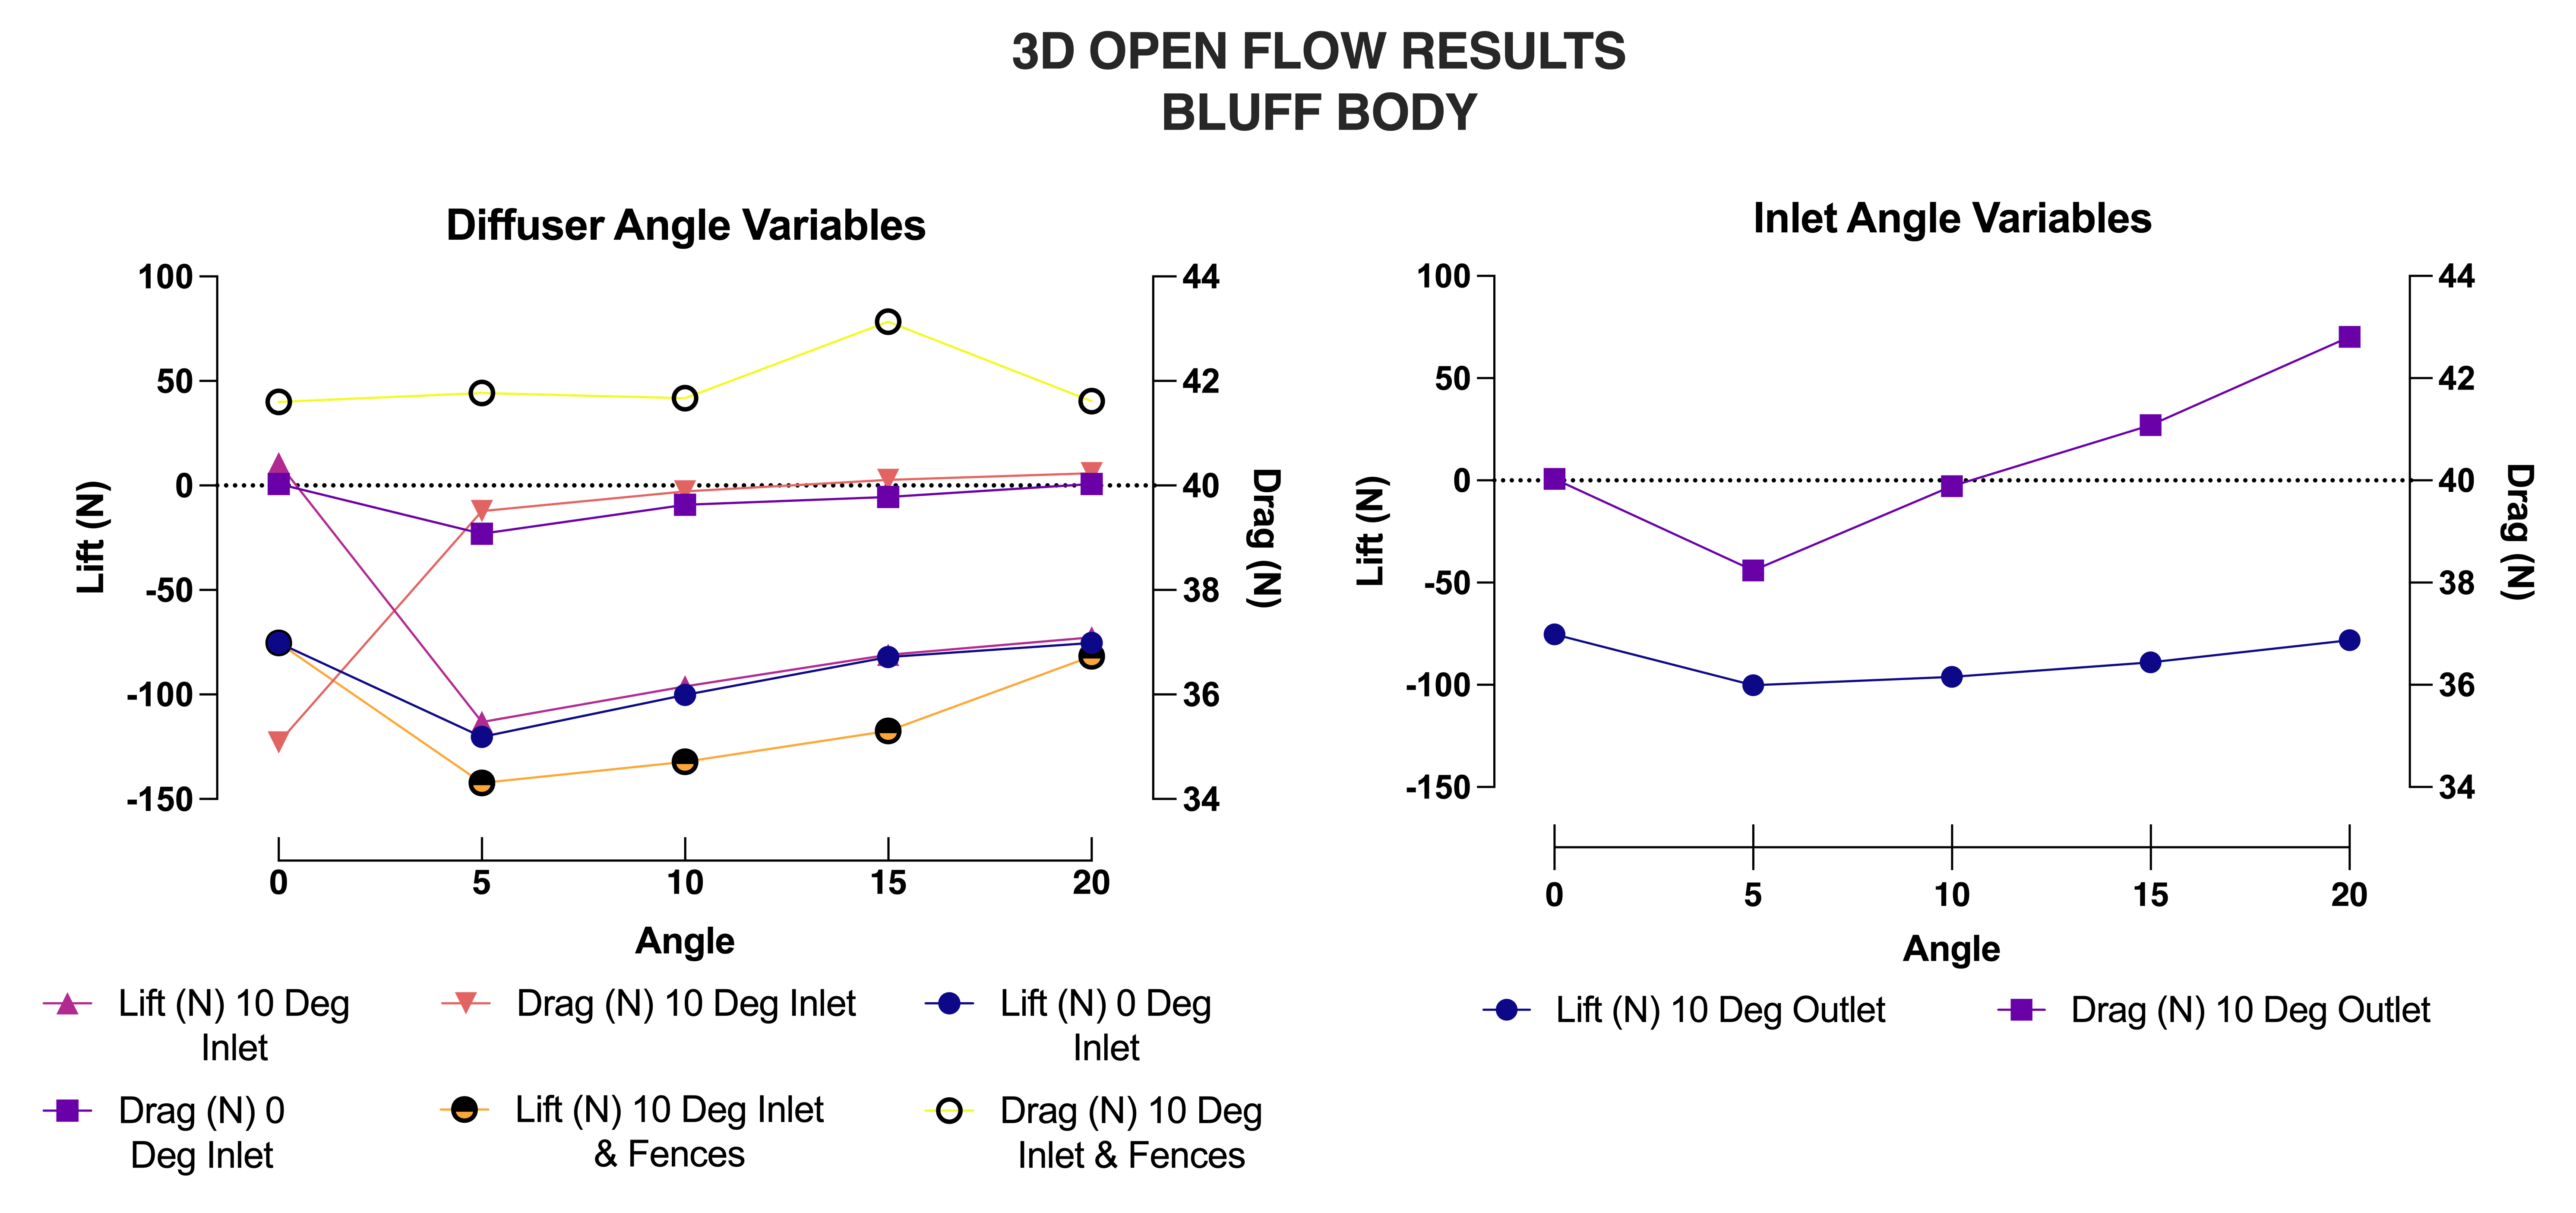
\includegraphics[width=0.9\textwidth]{Figures/Graph/3D_OF.png}}
    \caption{Lift and drag variation of diffuser (left) and inlet (right) angle for all geometry configurations.}
    \label{fig:3D_OF_PLOT_COMPARE_ALL}
\end{figure}

\noindent The value of lift and drag showed a representation of half bluff body as computed. Once more, a similar trend emerged compared to 2D open flow geometry 3 means the 2D bluff body, in this case can be deduced as the representation of the 3D analysis.  The trend shows an increase in downforce at a 5 degrees diffuser angle, followed by linear downforce reduction up to 20 degrees.  In comparison with 2D open-flow analysis, the average downforce of this analysis is significantly lower. This is due to the nature of the analysis that allows the accelerated flow in the undertray to be affected by the flow surrounding the body compared to the 2D open-flow, where the flow on the undertray is solely affected by the flow. This cause the lower pressure region in the undertray to suck in the air from the surrounding,  reducing the effectiveness of the flow acceleration underneath, hence lower downforce. This phenomenon is illustrated in figure \ref{fig:Vector_suction_diagram} below with influence of corner vortex occurred from the forepart of bluff body. 

\begin{figure}[!htb]
    \centering
    \noindent\makebox[\textwidth]{
    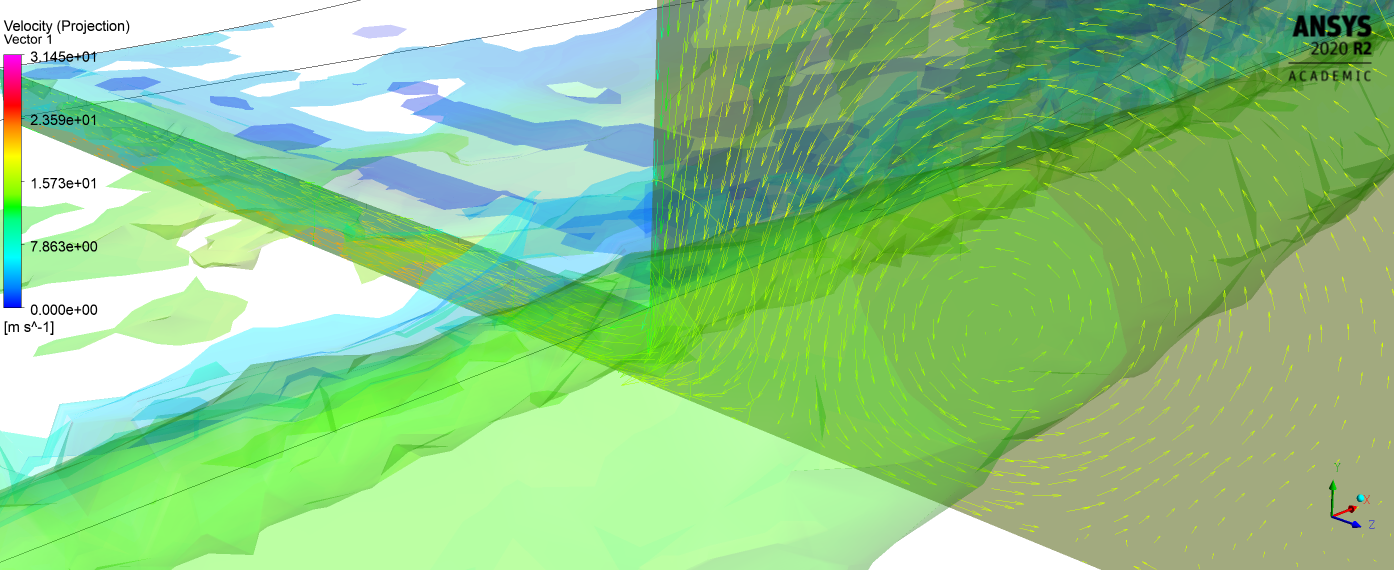
\includegraphics[width=0.8\textwidth]{Figures/3D_OF/3D_OF_VECTOR_SUCTION.png}}
    \caption{Vector diagram of velocity flow on the undertray's cross-section indicating flow suction from the side of the body.}
    \label{fig:Vector_suction_diagram}
\end{figure}

\noindent The inlet angle elevation was simulated with 10 degrees diffuser angle. It can be examined that the effect of inlet angle elevation shows significant difference to the 2 dimensional analyses. Lift and drag of the bluff body reach its minimum at 5 degrees which then followed by lift and drag rise up to 20 degrees. As discussed in earlier section, stagnation point in the forepart of bluff body in 2 dimensional simulation creates separation point of flow direction to the top and bottom. However, in 3 dimensional case, the stagnation point separates the flow without consistent direction which create more complex flow features in the inlet region. An identical front cross-section of the car was made on the fore-flow of the body which became the initial location of streamline. Figure \textbf{\ref{fig:3D_OF_INLET_COMPARE} left} shows the streamline separation from the free flow to the surrounding body. Moreover, some of the streamline flow are leaked to the side, creating a trailing corner vortex \textbf{(middle)} hence reducing the intake acceleration in the undertray.  Compared to the 2 dimensional analysis, the flow that goes to the undertray stays without leaking or generate trailing vortex, which make the flow intake better, hence higher downforce. This explains the downforce degradation after 5 degrees, as the inlet angle increases, more airflow are leaking on the inlet region and creating bigger trailing vortex. Increase in drag comes from the skin friction as the flow is imposed by larger area with elevation of angle, and the trailing vortex which plausibly affect the flow on the throat (as discussed previously). It is worth noting that the changes of drag with inlet angle elevation is not significant and can be ignored, hence it was not used in  bluff body geometry with fences.

\begin{figure}[!htb]
    \centering
    \noindent\makebox[\textwidth]{
    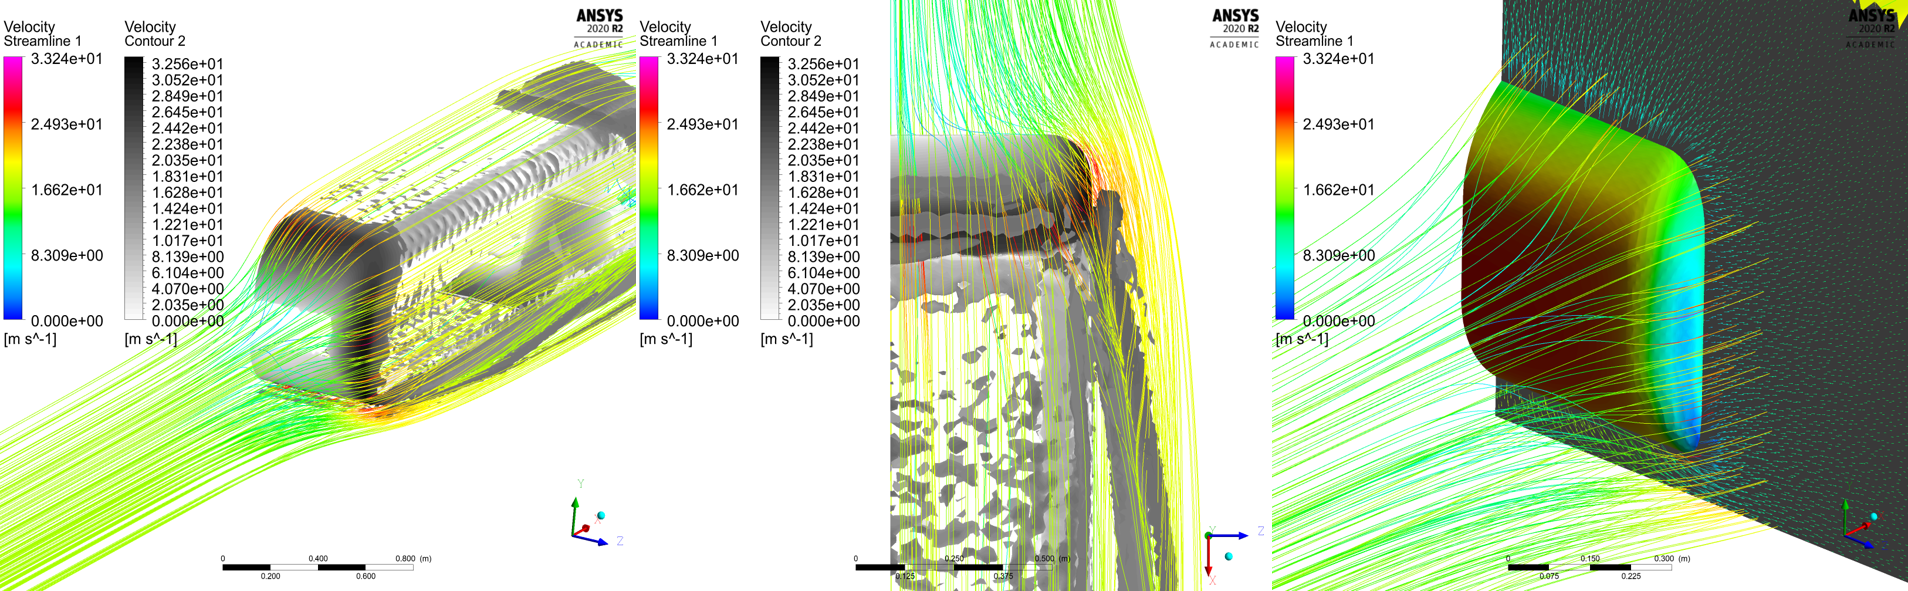
\includegraphics[width=1\textwidth]{Figures/3D_OF/3D_OF_INLET_COMPARE.png}}
    \caption{Fore-flow streamline imposing the bluff-body and occurrence of leaking indicated by the trailing vortex ($Q$-criterion isosurface) at the inlet region (left and middle), and velocity vector of the flow indicating flow leaks at the inlet region (right).} 
    \label{fig:3D_OF_INLET_COMPARE}
\end{figure}

\noindent Comparing the lift and drag for diffuser variable with or without inlet angle; the graph exhibit an identical result except at 0 degrees.  There is a noticeable drop in downforce and drag (however insignificant), which plausibly due to the diffuser's absence. A well-designed diffuser is important to slowly expand the flow and allows the jet flow to stay attached to the diffuser. Moreover, diffusers side skirts' presence allows the the generation of corner vortices that help the flow to attached, hence increasing the overall downforce.  ANSYS Post CFD allows the visualisation of Q-Criterion which shows a vortex region ($Q > 0$) where anti-symmetric component of vorticity tensor is more dominating than the symmetric \cite{Holmen2012MethodsIdentification}. The corner vortex allows the boundary layer to stick on the wall which slows the pressure expansion hence reduction in lift and drag. This phenomenon can be seen on \textbf{figure \ref{fig:3D_OF_COMPARE_FENCES_SHEAR}} where the the region where vortex is present has a higher wall shear than its surrounding which indicates flow attachment in the respective direction.

\begin{figure}[!htb]
    \centering
    \noindent\makebox[\textwidth]{
    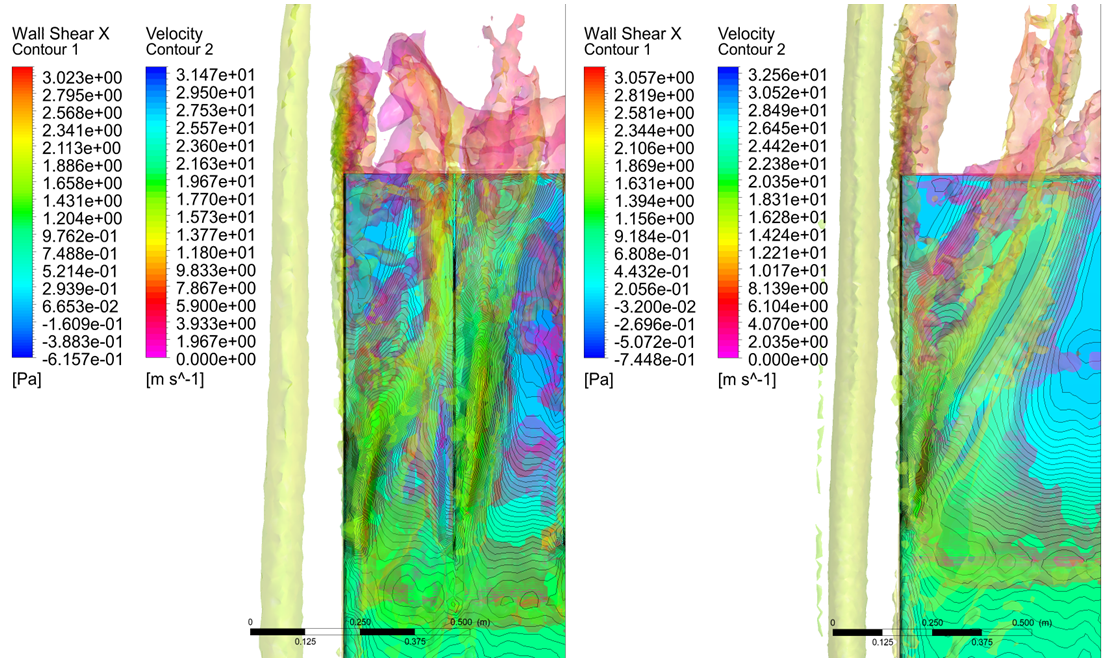
\includegraphics[width=0.65\textwidth]{Figures/3D_OF/3D_OF_COMPARE_FENCES.png}}
    \caption{Comparison of x-wall shear and vortex velocity (Q-criterion isosurface) generated on the diffuser region with (left) and without (right) fences applied.}
      \label{fig:3D_OF_COMPARE_FENCES_SHEAR}
\end{figure}

\noindent The next analysis will include fences (a vertical partition on a diffuser) to generate corner vortices and investigate its effect on the undertray's performance. The lift and drag plot on figure \ref{fig:3D_OF_PLOT_COMPARE_ALL} exhibit an overall higher downforce compared to the bluff body without the fences. Similar concept of vortex generation applies; as the fences installed, there are more vortex generated along the diffuser. This condition creates less flow separation in the x direction (flow direction), maintaining flow attachment, and increases the downforce. Figure \ref{fig:3D_OF_COMPARE_FENCES_SHEAR} illustrates the presence of more vortices generated inside the diffuser with additional fences, and smaller flow separation region indicated by non zero x-wall shear region. 

%TALK ABOUT SYMMETRY LIMITATION

\subsection{3D Undertray}
Overall previous analyses have given a fundamental understanding of flow behaviour, features, and performance trends of an underbody flow. This section of the report will utilise prior simulations to design several undertray prototypes that will be simulated using traced bluff-body of QFR car to achieve a sensible picture of the flow in real-life circumstances. The results documented then analysed thoroughly.

\subsubsection{Geometry and Mesh Generation}
\noindent Previous results have given knowledge on undertray's trend and flow behaviour for inlet and diffuser angle. Eight prototype designs were made based on interpretation and judgement from prior results. Number of configurations were used to achieve the best results in the designs, including; side diffuser, side flat-plate, dual-variable diffuser, Gurney flaps, and variable vortex generator. Those variables were designed to achieve the maximum performance of an undertray. All eight undertray prototype geometries can be seen on figure \ref{fig:UTP_D} in Appendix D.

\noindent The geometry then  vv 

\begin{figure}[!htb] %BODY SIMPLIFICATION DIAGRAM
    \centering
    \noindent\makebox[\textwidth]{
    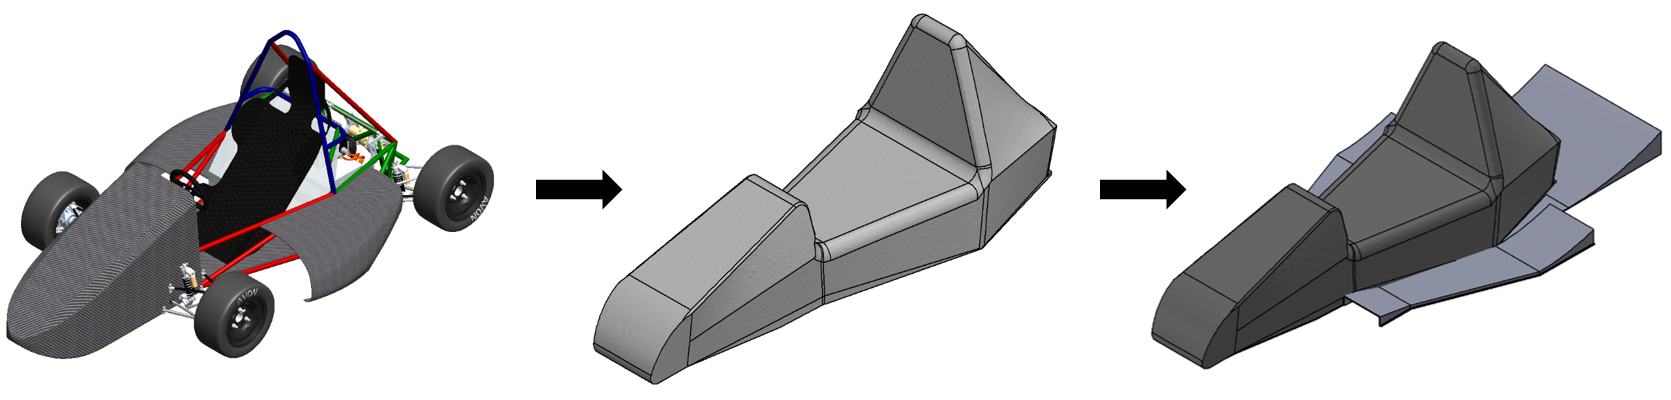
\includegraphics[width=0.7\textwidth]{Figures/UTP_FIGS/UT_BB_SIMPLIFY.png}}
    \caption{Simplification of QFR car as an undertray's Bluff Body to simulate realistic flow around the body.}
      \label{fig:3D_UT_BB_SIMPLIFICATION}
\end{figure}
\subsubsection{Results and Discussion}




















